%%####################################################################
%    Copyright @ 2007 Andreas Frieß (Friess)
%    Permission is granted to copy, distribute and/or modify this document
%    under the terms of the GNU Free Documentation License, Version 1.2
%    or any later version published by the Free Software Foundation;
%    with no Invariant Sections, no Front-Cover Texts, and no Back-Cover Texts.
%    A copy of the license is included in the section entitled ``GNU
%    Free Documentation License''.
%%####################################################################
% Created: 17.08.2007
% @cvs($Date: 2007-09-05 19:46:18 +0000 (Wed, 05 Sep 2007) $)
% @cvs($Rev: 38 $)
% @cvs($Author: af0815 $)
% @cvs($URL: file:///svn/p/lazsnippets/code/trunk/dokumentation/LazSnippets/Kapitel/datenbanken/HowToNewMySQL.tex $)
%%####################################################################
\subsection{Demodatenbank MySQL}

%%####################################################################
\subsubsection{Installieren von MySQL 5.x}
Am einfachsten ist es im Internet auf die MySQL-Seite\footnote{http://www.mysql.de/} zu gehen und dort unter "`Community"'\footnote{http://dev.mysql.com/} den Punkt "`Downloads"' und "`MySQL Community Server"' auszusuchen. Dort kann man sich dann den entsprechenden Server für sein Betriebssystem aussuchen und herunterladen. Die Dateigröße kann schon einen Breitband Internetzugang verlangen, denn je nach Version sind bis zu knappen 100 MB Download-Volumen gefragt.

Weiters ist es zu empfehlen, das man sich unter "`Downloads, GUI Tools"' auch noch die Programme "`MySQL Administrator"' und "`MySQL Query Browser"' herunterlädt. Mit Hilfe der beiden Tools kann man später dann den Server komfortabel administrieren und auch die Datenbanken verwalten und Scripts laufen lassen. Die Tools sind nicht zwingend erforderlich, erleichtern aber gerade am Anfang das Leben. 

Eine Alternative dazu ist sicherlich auch das arbeiten mit "`PHPMySQLAdmin"'. Das Tool ist sehr ausgereift und auch entsprechend bekannt. Ein Nachteil dabei ist, das es einen Webserver mit PHP voraussetzt.

Zur Installation geht man entsprechend den Erfordernissen seines Betriebssystems vor. Es würde den Rahmen dieser Beschreibung sprengen, für jedes Betriebssystem mit seinen Eigenheiten eine entsprechende Anleitung zu erstellen.

Wichtig ist nur, das man bei der Installation  und Konfiguration nicht vergisst, ein gutes Passwort für den "`root"' ("`Administrationsuser"') zu wählen. Denn später vergisst man gerne den laufenden MySQL-Server und wenn der Rechner dann doch im Internet auftaucht, so hat man ein ganz schönes Sicherheitsleck, das einem gar nicht bewusst ist. Dasselbe gilt natürlich in abgemilderter Form auch für normale Benutzer, die etwas mehr Rechte als lesen in der Datenbank haben. Eine gute Möglichkeit ist, ein launiges Sprichwort zu nehmen und die Anfangsbuchstaben aneinander zu reihen. Beispiel: "`Wir sind ja nicht blöd Mann und haben 99 Luftballone gekauft"'. Daraus kann sich ein Paßwort wie folgt ergeben "`WsjnbMuh99Lg"'. Das lässt sich noch so halbwegs merken und besteht aus Groß\- und Kleinbuchstaben, beinhaltet Zahlen und ist außerdem noch zwölf Zeichen lang. 

Aber genug dem Ausflug in die Installation und Paßwortauswahl, beginnen wir nun mit der Erstellung unserer Datenbank, die sich dann später durch alle Beispiele ziehen wird.

%%####################################################################
\subsubsection{Erstellung der DEMO Datenbank}
Das Erste, das wir am neuen oder geleerten MySQL Datenbankserver erstellen, ist eine neue Datenbank für unsere Zwecke. Dazu öffnen wir den "`MySQL Query Browser"'.
\parpic[sl][r]{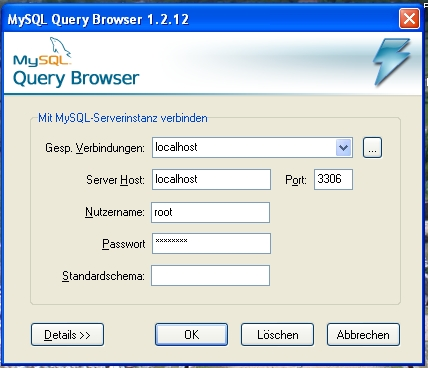
\includegraphics[width=0.3\textwidth]{Kapitel/datenbanken/pics/NewDB01}}
%\parpic[lf][r]{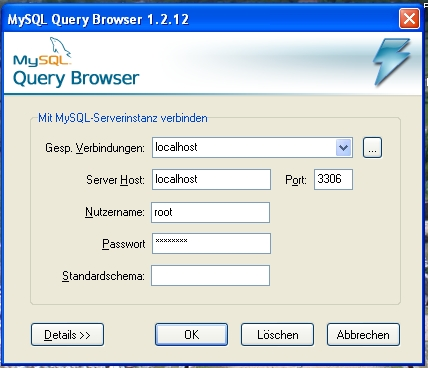
\includegraphics[width=6cm,height=6cm]{Kapitel/datenbanken/pics/NewDB01}}
%\caption[NewDB01]{Verbindungsdialog}
\label{fig:NewDB01}
%\begin{figure}[tp]
%\centering
%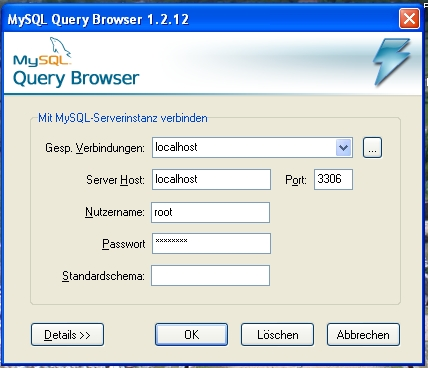
\includegraphics[totalheight=0.3\textwidth]{Kapitel/datenbanken/pics/NewDB01}
%\caption[NewDB01]{NewDB01}
%\label{fig:NewDB01}
%\end{figure}
Es öffnet sich als ersters das Verbindungsfenster. Ich werde jetzt die Felder von oben nach unten besprechen, denn es könnte ja sein, das sie eine andere Sprachversion verwenden. 

Unter "`Gesp. Verbindungen"' wird ein beliebiger Namen eingetragen, unter der später die Einstellungen wieder abgerufen werden können. Bei "`Server Host"' und "`Port"' geben wir, bei einer lokalen Installation, "`localhost"' und "`3306"' ein. Wobei die Portnummer "`3306"' der Standardport von MySQL ist. Als nächstes kommen jetzt der "`Nutzername"' und das "`Passwort"' dran, dort geben wir in diesem Fall den Benutzer "`root"' mit dem bei der Installation vergebenen Paßwort ein. Später sollte man sich nur in zwingend notwendigen Fällen mit dem Administratorpaßwort verbinden. Das Feld "`Standardschema"' lassen wir bei diesem ersten Einstieg einmal leer.
\parpic[sr][r]{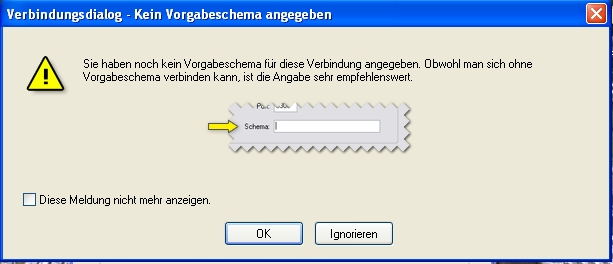
\includegraphics[width=0.3\textwidth]{Kapitel/datenbanken/pics/NewDB02}}
%\caption[NewDB02]{Fehlendes Standardschema}
\label{fig:NewDB02}

Anschliessend gehen wir mit "`Ok"' im Dialog weiter, das nun folgende Hinweisfenster zum Thema fehlendes Standardschema übergehen wir mit dem Button "`Ignorieren"'. Ist bis jetzt alles gut verlaufen und der MySQL Datenbakserver aktiv, so öffnet sich jetzt endgültig der "`MySQL Query Browser"'.

\parpic[sl][r]{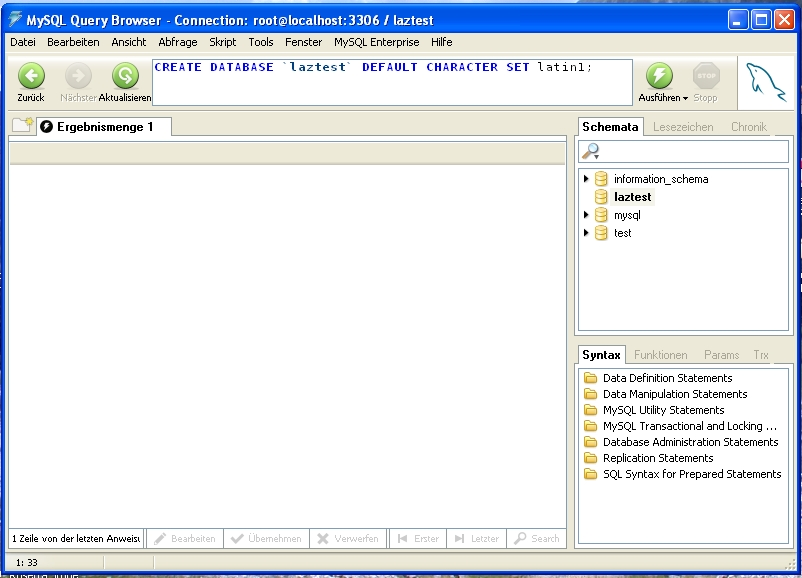
\includegraphics[width=0.3\textwidth]{Kapitel/datenbanken/pics/NewDB03}}
\label{fig:NewDB03}
Als ersters erzeugen wir mittels \textbf{\emph{CREATE USER lazarus@localhost IDENTIFIED BY 'WsjnbMuh99Lg';}} einen neuen Benutzer, der noch dazu ein halbwegs sicheres Paßwort hat. Zusätzlich geben wir diesen Benutzer alle Recht an dieser Datenbank mit folgenden Befehl \textbf{\emph{GRANT all ON *.* TO lazarus@localhost;}}. Somit hat der Benutzer alle Rechte außer dem Recht, selbst Rechte zu vergeben.

Im Menüpunkt "`Datei"' wählen wir die Funktion "`Verbindung umschalten"' an und wechseln die Verbindung auf den User "`lazarus@localhost"'. Alternativ kann man den "`MySQL Query Browser"'  schliessen und als Benutzer "`lazarus"' neu anmelden. Damit wir nicht immer die Informationen neu eingeben müssen, kann man den Button rechts neben den "`Gesp. Verbindungen"' benutzen und sich dort ein entsprechndes Profil anlegen. Somit braucht man später nur sein Profil in der Top-Down Box anwählen, das Paßwort eingeben und schon ist man drinnen. 

Anschließend erzeugen wir jetzt als Benutzer "`lazarus@localhost"' mittels dem Kommando \textbf{\emph{CREATE DATABASE `laztest` DEFAULT CHARACTER SET latin1;}} eine neue Datenbank, mit dem Namen "`laztest"'. Diese Zeile geben wir oben im "`MySQL Query Browser"' ein und drücken dann auf den grünen Button daneben. Anschließend können wir mit der Maus auf "`Schemata"' klicken und mit der Taste "`F5"' ein neuerliches einlesen der Übersicht der Datenbanken (= Schemata) erreichen. Jetzt sollte dort unsere neue Datenbank vorhanden sein.  

Somit haben wir die Datenbank erstellt und auch einen Beutzer mit hohen Rechten darin erzeugt. Für den produktiven Betrieb würde sich jetzt noch anbieten, einen Benutzer zu erzeugen, der entsprechend den Erfordernissen weniger Rechte hat. Aber nachdem das hier ja ein Tutorium ist, belassen wir es einmal dabei.

\subsubsection{Windows FAQ}
\paragraph{Einleitung}
Es hat sich auch bei mir gezeigt, das es manchmal nicht so einfach ist, MySQL unter Lazarus zu verbinden. Hier ein paar Hilfen.

\paragraph{Cannot load MySQL library "`libmysql.dll"'}
Dieser Fehler kann mehrer Ursachen haben. Die einfachste ist, dass auf dem Rechner ganz einfach die Treiber für MySQL nicht installiert sind. 
\parpic[sr][r]{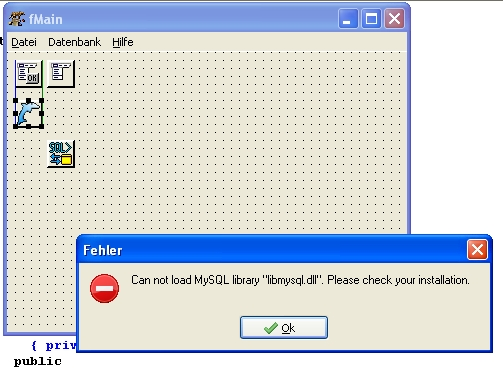
\includegraphics[width=0.3\textwidth]{Kapitel/datenbanken/pics/FAQWDB01}}
\label{fig:FAQWDB01}
Die Abhilfe ist die Datei in ein Verzeichnis, dass sich im Suchpfad befindet zu kopieren. Genauso ist es möglich, die Bibliothek ins selbe Verzeichnis wie die ausführbare Datei zu kopieren, der Weg bietet sich an, wenn es an den Rechten am Systemverzeichnis fehlt.

Wenn das ganze, wie am Bild, innerhalb von Lazarus passiert, so kann es einmal am Lazarus liegen. Besonders wenn man eine Version aus dem SVN selbst kompiliert, kann es vorkommen, das es hier Probleme gibt. Die Abhilfe ist nur, eine bessere oder stabile Version von Lazarus zu verwenden. 
Genauso kann es sein, dass wie oben bereits besprochen, die Biblothek fehlt. Die Abhilfe ist wieder die Biblothek in ein Verzeichnis, dass im Suchpfad liegt zu kopieren. Geht das nicht, so muß die Datei einmal in des Verzeichnis kopiert werden, wo sich die "`Lazarus.exe"' befindet und einmal in das Verzeichnis, wo die ausführbare Datei des Projektes liegt. Denn innerhalb der IDE benötigt Lazarus die Datei in seinem Pfad, wird die Datei aber ausgeführt, so benötigt sie das aktuelle, kompilerte und gestartete Programm.

\verb|Version: $LastChangedRevision: 38 $ |\footnote{ Autor: Andreas Frieß\\Lizenz: GFDL}